%%%%%%%%%%%%%%%%%%%%%%%
% Section 3
% 17/03/2026
% fclinquart 
%%%%%%%%%%%%%%%%%%%%%%

\begin{frame}{End of life route}
    \begin{itemize}
        \item No Biodegradability 
        \item No chemical recycling : Polymerization always $\Delta G < 0$ 
        \item Mechanical recycling
        \item Mismanagement
        \item Thermo-degradation to form fuel \cite{jubinville_comprehensive_2020}. 
    \end{itemize}
\end{frame}

\begin{frame}
    \frametitle{What happens to the polymer structure ? }
    According to \textcite{ragaert_mechanical_2017} :
    \begin{block}{}
        \begin{enumerate}
        \item Re-extrusion step
        \item The use phase
    \end{enumerate}
    \end{block}

    Degradation mechanisms:
    \begin{center}
        \begin{itemize}
        \item \textbf{Thermo-mechanical degradation.}
        \item Thermo-oxidative degradation.
        \item Hydrolytic degradation.
        \item \textbf{Impurities and contaminants.}
    \end{itemize}
        
    \end{center}
\end{frame}

\begin{frame}
\frametitle{leading to two thermo-mechanical degradation mechanisms}
\begin{figure}
    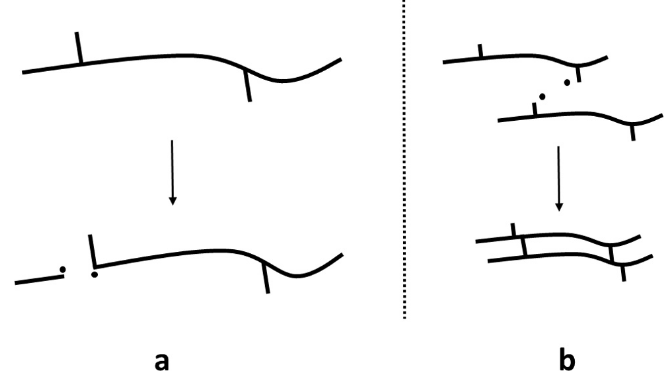
\includegraphics[width=0.5\textwidth]{Figures/thermo-mechanical.png}
    \caption{Random chain scission (a) and cross-linking (b)  \cite{ragaert_mechanical_2017}.}
\end{figure}
\begin{alertblock}{}
    \textbf{$M_w \downarrow$ or $M_w \uparrow$ } and $M_w$ $\infty$ $E$, $\sigma_Y$, $\epsilon_{break}$, $\sigma_{Impact}$, $\chi_{c}$ and $\mu$. 
\end{alertblock}
\end{frame}

\begin{frame}
    \frametitle{Polyolefins behave very differently during mechanical recycling.}
    \begin{minipage}{0.45\textwidth}
\begin{figure}
    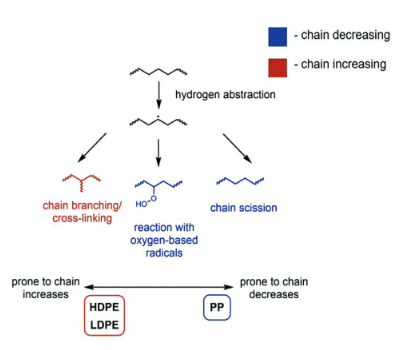
\includegraphics[width=0.8\textwidth]{Figures/polyolefin.png}
    \caption{General reaction scheme of polyolefins undergoing extrusion.}
\end{figure}
\end{minipage}
\hfill
\begin{minipage}{0.45\textwidth}
\begin{figure}
    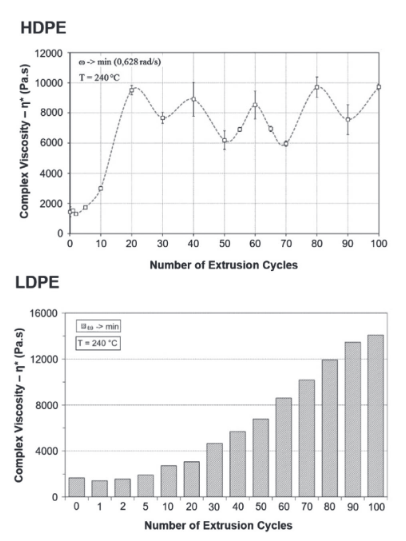
\includegraphics[width=0.8\textwidth]{Figures/complex_viscosity.png}
    \caption{Complex viscosity versus number of extrusion cycles.}
\end{figure}
\end{minipage}

\end{frame}


\begin{frame}{Effect of Recycling on Polyolefin Properties}
    \begin{table}[h]
        \centering
        \small
        \begin{tabular}{l c c c}
            \toprule
            \textbf{Property} & \textbf{Typical Effect} & \textbf{HDPE} & \textbf{PP} \\
            \midrule
            Molecular Weight & ↓ (chain scission) & vary & ↓ Significant \\
            PDI & Changes & ↑ Increases & ↓ Decreases \\
            Tensile Strength & ↓ Loss & 10-30\% & 10-30\% \\
            Crystallinity & ↓ Loss & 5-10\% & 5-10\% \\
            Melt Flow Index (MFI) & ↑ Increases & More fluid & More fluid \\
            ESCR & ↓ Loss & 60\% reduction & — \\
            \bottomrule
        \end{tabular}
        \caption*{Loss of properties \cite{jubinville_comprehensive_2020} \small ESCR: Environmental Stress Crack Resistance}
    \end{table}
\end{frame}

\begin{frame}{Pyrolysis}
    making oil 
\end{frame}

\begin{frame}{Chemical recycling}
    need catalyst and not mature
\end{frame}

\begin{frame}{Sorting problem}

\end{frame}

\begin{frame}{PE/PP blend}

\end{frame}

\begin{frame}{Too many grades}

\end{frame}

